\documentclass[tikz, 11pt]{standalone}

% Parameters and settings
\usetikzlibrary{shapes.geometric, arrows.meta, snakes, calc, decorations.pathmorphing}

% Styles
\tikzstyle{panel}=[draw=none, inner sep=0]
\tikzstyle{label}=[draw=none, anchor=north west, text height = 10pt, text depth=5pt]
\tikzstyle{lines}=[line width=0.75pt]
\tikzstyle{linesShort}=[lines, shorten > =1mm, shorten < =1mm]
\tikzstyle{headingNode}=[draw=none, inner sep=1mm, text height=7pt, text depth=1pt, fill=white]
\tikzstyle{textNode}=[draw=none, inner sep=1mm]

% Packages
\usepackage{amsmath,amssymb}
\usepackage[scaled]{helvet}
\renewcommand\familydefault{\sfdefault} 

% Font sizes
\newcommand{\tinySize}{\tiny}				% tiny corresponds to 6 pt
\newcommand{\textSize}{\scriptsize}		% scriptsize corresponds to 8 pt
\newcommand{\headingSize}{\small}		% small corresponds to 10 pt
\newcommand{\labelSize}{\large \bf}		% Large corresponds to 12 pt and bf for bold face

% Colors
\definecolor{discColor}{rgb}{1.0, 0.0, 0.0}
\definecolor{detColor}{rgb}{0.16, 0.16, 0.78}
\definecolor{onColor}{rgb}{0.37, 0.84, 0.0}
\definecolor{offColor}{rgb}{0.84, 0.12, 0.84}
\definecolor{psychoColor}{rgb}{1.0, 0.64, 0.02}
%\definecolor{modelColor}{rgb}{0.6, 0.25, 0.0}

\colorlet{retinaColor}{gray!25!white}
\colorlet{offEdgeColor}{offColor}
\colorlet{onEdgeColor}{onColor}
\colorlet{boxColor}{gray!20!white}
\newcommand{\fillSat}{40}
\renewcommand{\textSize}{\scriptsize \baselineskip=8pt}

\begin{document}
\begin{tikzpicture}[]

% Panels
\coordinate[] (topleft) at (0, 0);
\node[panel, anchor=north west, xshift=1mm] (a) at (0cm, 0cm) {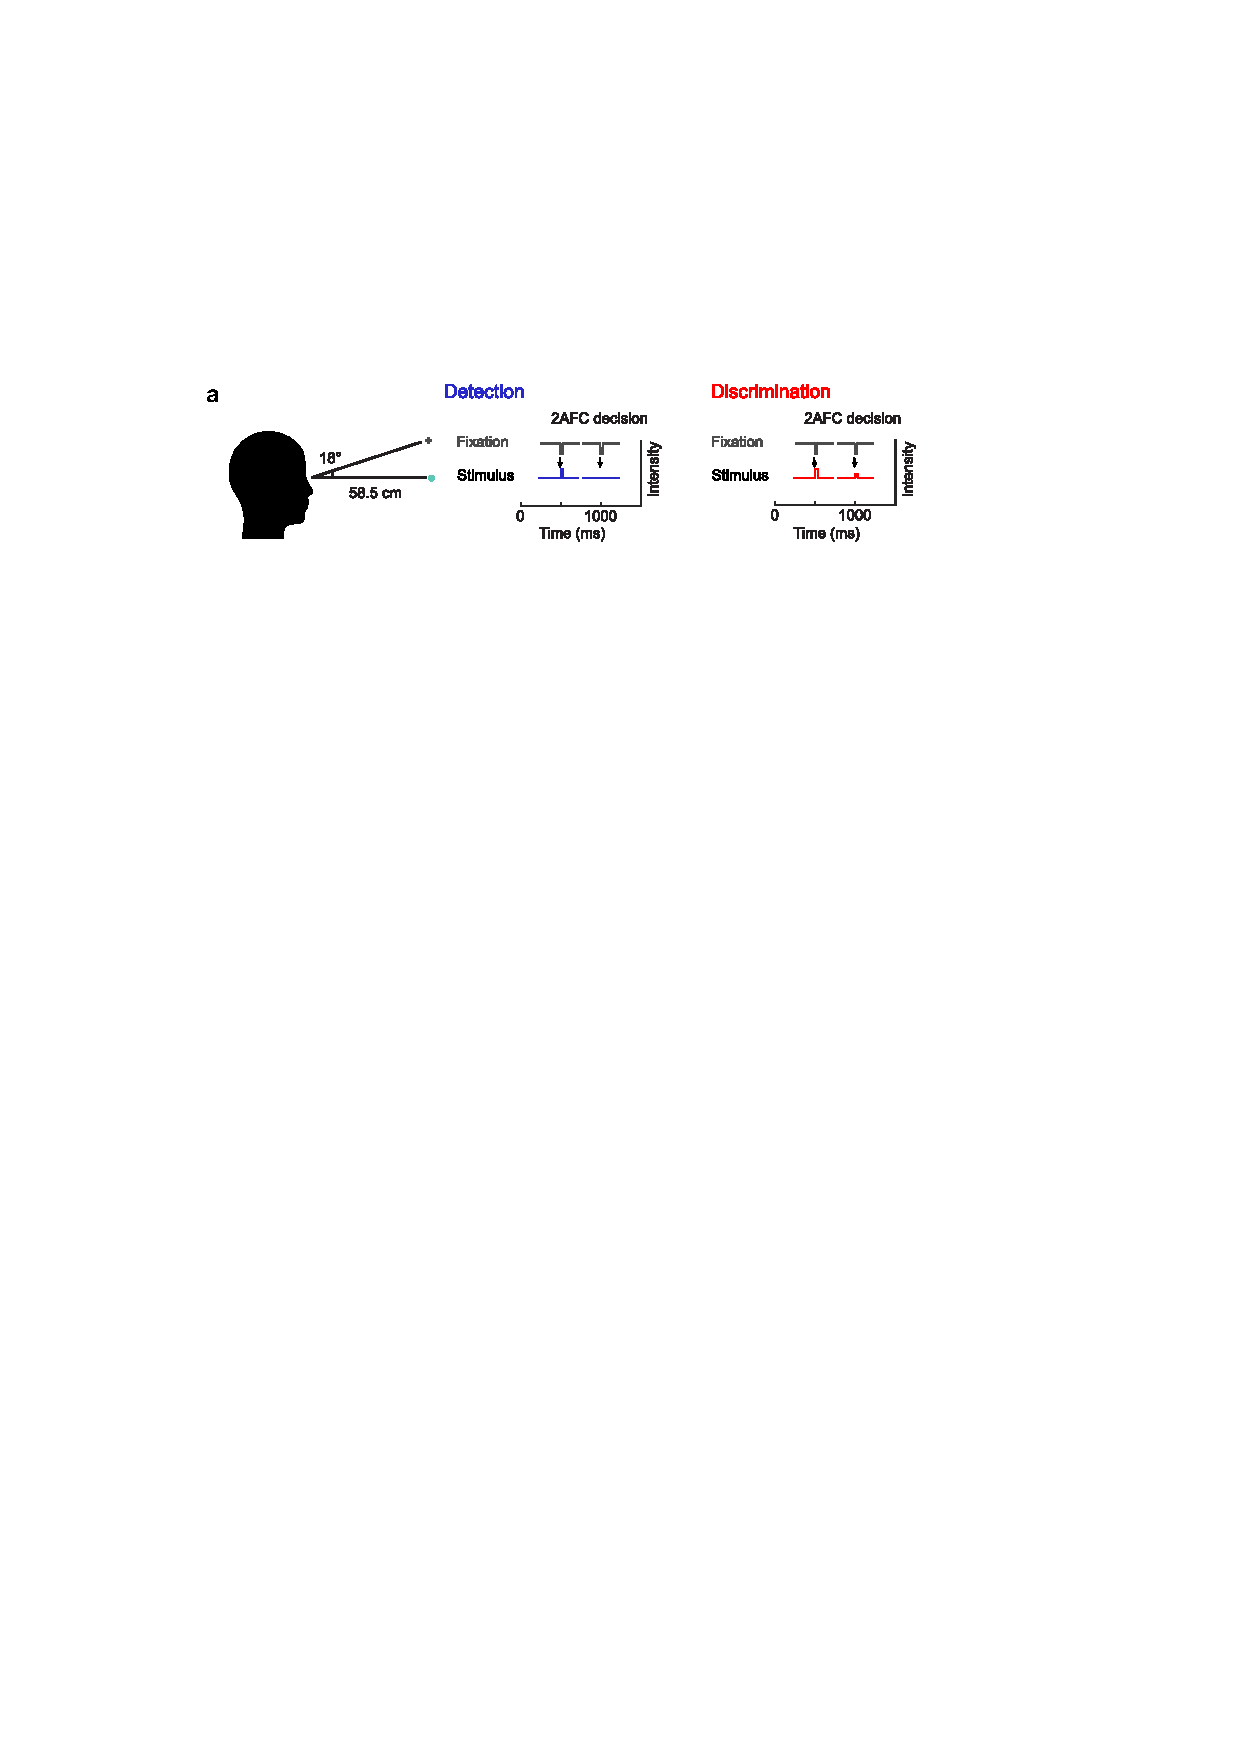
\includegraphics[trim=37mm 205mm 54mm 65mm, clip]{Fig3a}};
\node[panel, anchor=north west] (b) at (a.south -| topleft) {\includegraphics{"../Figure Panels/Fig3_Psycho2AFC"}};
\node[panel, anchor=north west] (c) at (b.north east) {\includegraphics{"../Figure Panels/Fig3_PsychoDippers"}};
\node[panel, anchor=north west, yshift=-17mm] (d) at (b.south west) {\includegraphics{"../Figure Panels/Fig3_PsychoRGCDipper"}};
\node[panel, anchor=north east, yshift=-17mm] (e) at (c.south east) {\includegraphics{"../Figure Panels/Fig3_PsychoRGCDipperModel"}};

\newcommand{\dy}{3mm}
% Data icons
\node[panel, anchor=south west, xshift=14mm, yshift=-\dy-0mm] (off) at (d.north west) {\includegraphics{"Rod-Bipolar-Pathway/Rod-Bipolar-Off"}};
\node[panel, anchor=south west, xshift=29mm, yshift=-\dy-0mm] (on) at (d.north west) {\includegraphics{"Rod-Bipolar-Pathway/Rod-Bipolar-On"}};
\node[panel, anchor=north, xshift=3.5mm, yshift=-0mm] (psycho) at (off.north east) {\includegraphics[]{"Icons/MonkeyIcon"}};
%\node[panel, anchor=north east, xshift=-6mm, yshift=0mm] (psycho) at (d.north east |- on.north) {\includegraphics[]{"Icons/PsychoPhysicsIcon"}};
\node[panel, anchor=north east, xshift=-7mm, yshift=0mm] (psycho) at (d.north east |- on.north) {\includegraphics[height=0.8cm]{"Icons/HumanIcon"}};
\node[panel, anchor=south, inner sep=0.5mm, text height=7pt, text depth=1pt] (psychoText2) at (psycho |- on.south) {\textSize \color{psychoColor} physics};
\node[panel, anchor=south, inner sep=0.5mm, text height=7pt, text depth=1pt, yshift=-1mm] (psychoText1) at (psychoText2.north) {\textSize \color{psychoColor} Psycho-};

% Model icons
\node[panel, anchor=west, xshift=14mm, yshift=1] (m1) at (e.north west |- on) {\includegraphics{"Models/Model1"}};
\node[panel, anchor=east, xshift=-1mm, yshift=1] (m3) at (e.north east |- on) {\includegraphics{"Models/Model2"}};

% Headings
\draw[draw=black, line width=1pt, shorten > =3mm, shorten < =3mm] (0,3mm) -- (12cm, 3mm) node [midway, headingNode] {\headingSize Human psychophysics};
\draw[draw=black, line width=1pt, shorten > =3mm, shorten < =3mm] (b.south west) --++ (6cm, 0) node [midway, headingNode] {\headingSize Data summary};
\draw[draw=black, line width=1pt, shorten > =3mm, shorten < =3mm] (b.south east) --++ (6cm, 0) node [midway, headingNode] {\headingSize Model vs. data};

% Labels
\node[label, yshift=1mm] at (a.north -| topleft) {\labelSize a};
\node[label, yshift=-2mm] at (b.north west) {\labelSize b};
\node[label, yshift=-2mm] at (c.north west) {\labelSize c};
\node[label, yshift=12mm] at (d.north west) {\labelSize d};
\node[label, yshift=12mm] at (e.north west) {\labelSize e};

\end{tikzpicture}
\end{document}